\documentclass{beamer}
\usepackage{hyperref}
\usepackage{graphicx}
\usepackage{amssymb}
\usepackage{amsmath}
\usepackage{anyfontsize}

%%%%%%%%%%%%%%%%%%%%%%%%%%%%%%%%%%%%%%%%%%%

\title{INTRO TO AI AND ML}
\subtitle{(EE1390)}
\author{MATRIX PROJECT}

\date{14 Feb 2018}
\institute{G.NAGA DHANUSH , EE17BTECH11014 \and B.GOWRI SHANKAR REDDY , EE17BTECH11009}
\begin{document}

\begin{frame}
	
	\titlepage
	
\end{frame}

\begin{frame}[t] {PROBLEM:31}

A variable line drawn through the intersection of lines


   
    $\begin{bmatrix}
    4 & 3
    \end{bmatrix}$X=12


    $
    \begin{bmatrix}
    3 & 4
    \end{bmatrix} $X  = 12
    
meets the cordinate axes at A and B,then find the locus of the mid point.

\end{frame}

\begin{frame}{Solution}
The given linear equations are


$
\begin{bmatrix}
    4 & 3 \\
    3 & 4
\end{bmatrix}
$X =    
     $\begin{bmatrix}
    12 \\
    12
    \end{bmatrix}$ 
    
Let P =   
 $\begin{bmatrix}
   4 & 3 \\
   3 & 4
    \end{bmatrix}$,
        
    Q= $\begin{bmatrix}
    12 \\ 
    12
   
    \end{bmatrix}$    

PX = Q

X = $P^{-1}$Q

X is point of intersection

X =
 $  
\begin{bmatrix}
  
1.714 \\
1.714
\end{bmatrix}
$;
    
    

    
\end{frame}

\begin{frame}
Variable lines passing through X is




 $\begin{bmatrix}
 m &-1 
\end{bmatrix}$X =1.714(m-1)


where m is paramter


It meets cordinate axes at A and B respectively
 
A=$\begin{bmatrix}
  
a\\
0
    \end{bmatrix}$
B=$\begin{bmatrix}
  
0\\
b
    \end{bmatrix}$

a = 1.714$\frac{m-1}{m}$,
b = 1.714(1-m)
    
The locus of midpoint of A and B is C
    
    C=$\begin{bmatrix}
  
x\\
y
    \end{bmatrix}$


x,y are $\frac{a}{2}$ and $\frac{b}{2}$  respectively


x = $\frac{0.8571(m-1)}{m}$,y = 0.8571(1-m)


$\frac{y}{x}$ = -m

xy = 0.8571(x+y)

Therefore the locus is a hyperbola whose equation is
C=$\begin{bmatrix}
  
0.8571(m-1)/m\\
0.8571(1-m)
    \end{bmatrix}$


m is parameter.
\end{frame}

\begin{frame}
\textbf{FIGURES}


The figure of locus diagram
\begin{figure}
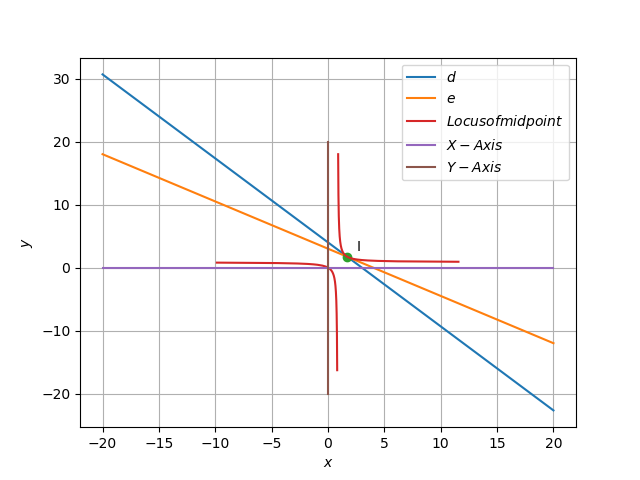
\includegraphics[scale=0.5]{locus}
\caption{locus diagram}
\end{figure}

\end{frame}
\begin{frame}
The figure of variable lines
\begin{figure}
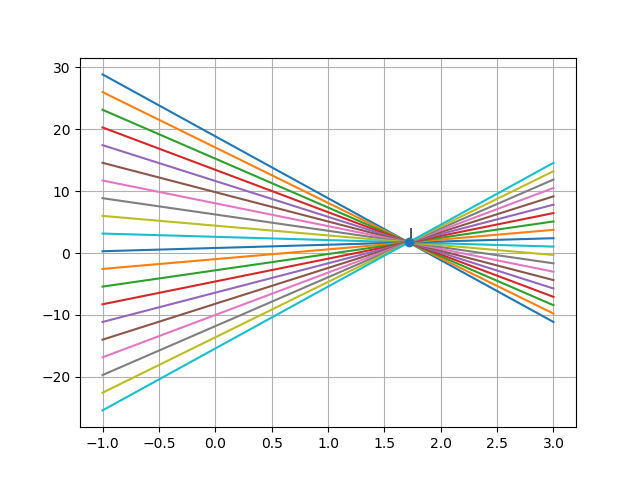
\includegraphics[scale=0.5]{variable_lines}
\caption{variable lines}
\end{figure}

\end{frame}
\end{document}




